% This is LLNCS.DEM the demonstration file of
% the LaTeX macro package from Springer-Verlag
% for Lecture Notes in Computer Science,
% version 2.4 for LaTeX2e as of 16. April 2010
%
\documentclass{llncs}
%
\usepackage{graphicx}
\usepackage{amsmath}
\PassOptionsToPackage{hyphens}{url}\usepackage{hyperref}
%\RequirePackage[hyphens]{url}

\usepackage{biblatex}
\bibliography{references.bib}

%\usepackage{makeidx}  % allows for indexgeneration
%
\begin{document}
%
\frontmatter          % for the preliminaries
%
\pagestyle{headings}  % switches on printing of running heads
\addtocmark{Non-Parametric Transformation Networks} % additional mark in the TOC
%
\mainmatter              % start of the contributions
%
\title{Non-Parametric Transformation Networks \\Lab: Cognitive Robotics}
%
\titlerunning{Non-Parametric Transformation Networks}  % abbreviated title (for running head)
%  
%
\author{Daniel Biskup and Catherine Capellen
 \\Supervisors: Arul Selvam and Max Schwarz}
%
\authorrunning{Daniel Biskup and Catherine Capellen} % abbreviated author list (for running head)
%
%%%% list of authors for the TOC (use if author list has to be modified)
\tocauthor{Daniel Biskup and Catherine Capellen}
%
\institute{University of Bonn}

\maketitle              % typeset the title of the contribution

\begin{abstract}
The abstract 
\end{abstract}
%

\section{Introduction}
Convolutional Neural Networks (CNNs) are state of the art in image classification tasks [FIND CITE]. Certain kind of transformations on these images do not affect the class of the depicted object. 
Examples for this are small rotations, translations or perspective transforms.  
Using augmented data in training as well as choices in the architecture of CNNs as pooling layers, aim to improve the robustness of CNNs to specific transformations. 
Pooling is a method that is usually performed spatially, to obtain invariance to small translations. 
Non-Parametric Transformation Networks (NPTNs) are extensions of CNNs, which use pooling to achieve invariance to other transformations by pooling over layers, rather than separately on the different layers.
Pal and Savvides \cite{NPTN} introduced NPTNs and performed experiments to test NPTNs against CNNs. The main objective of our project was to verify the results from the paper. 
Inspired by the NPTNs we additionally designed a network architecture, which we called RotNet, supposed to be invariant specifically towards rotations.

First we will describe the network architectures in more detail in Section [REF], then describe our implementation [REF] and experiments [REF] and lastly our Results [REF] and Conclusions [REF].

\section{Networks Architectures}
The kinds of networks this report is concerned with are Convolutional Neural Networks (CNNs), Non-Parametric Transformation Networks (NPTNs), a custom network architecture we call RotNets.

\subsection{Convolutional Neural Networks}
NPTNs can be seen as a generalization of CNNs. For that reason we will briefly discuss CNNs. 
\subsubsection{Convolution}
As the name suggests, NPTNs make heavy use of the convolution operation. Convolutions, as illustrated in Figure \ref{fig:conv}, calculate the weighted sum over a sub region of an input image in order to calculate the pixel-values of the output. The weights used for computing the weighted sum are given by a matrix called filter or kernel. In Computer Vision they are used to detect different kinds of patterns, since convolving an image with a kernel will produce high responses at the regions that match the pattern the filter is designed to respond to. Thus one kernel might respond to vertical edges, another  one to horizontal edges and yet another one to yet another pattern. While kernels traditionally got designed by experts in Computer Vision, within CNNs they are expected to be learned by the network.
\begin{figure}
	\begin{center}
		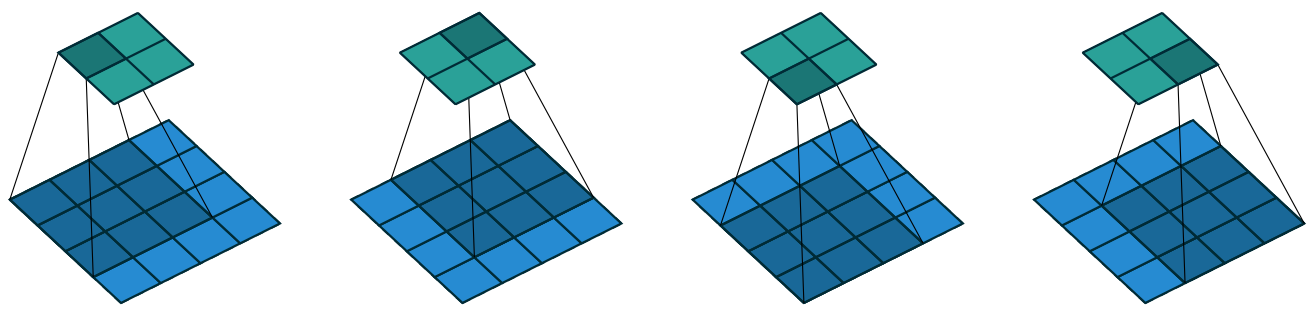
\includegraphics[width=\textwidth]{result_images/Conv.png}
		\caption{Convolving a 3 $\times$ 3 kernel over a 4 $\times$ 4 input using unit strides (Figure taken from \cite{ConvArithmetic16})}
		\label{fig:conv}
	\end{center}
\end{figure}

\subsubsection{Spatial Max Pooling}
Spatial max pooling, generally just called max pooling is another common operation used in CNNs.
Each neuron in the max pooling layer takes into account only a subregion of the previous
layers output and takes the maximum value of it to be it's output. By doing this it makes the network invariant to small translations. Max pooling is illustrated in Figure \ref{fig:maxpooling}.

\begin{figure}
	\begin{center}
		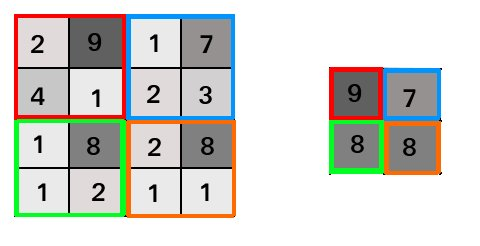
\includegraphics[width=0.40\textwidth]{result_images/maxpooling.jpg}
		\caption{Example of max pooling over a 4 $\times$ 4 image with a window size of $2 \times 2$ and a stride of $2$ [MORE]}
		\label{fig:maxpooling}
	\end{center}
\end{figure}

\subsection{Parametric and Non-Parametric Transformation Networks}

Parametric Transformation Networks (PTNs) and Non-Parametric Transformation Networks, as introduced in \cite{NPTN18}, try to add more transformation invariance to CNNs. For this a transformation group G is used:
Where a CNNs have one filter, PTNs and NPTNs have $|G|$ filters and a pixel wise max pooling operation is performed over the filters, such that for each pixel the strongest result of the convolution with a filter is used. This is illustrated in Figure \ref{pic:nptn}.

For the PTNs these $|G|$ filters are transformations of a base filter with weights $w$. The transformations belong to a (unitary) group of transformations G and are learned simultaneously to $w$ for each of the different $w$. 

For NPTNs the filters are independent of each other and are not restricted to belong to a transformation group. However they are expected to learn transformations.
For $|G|=1$ a NPTN conceptually does the same as a CNN, which is why NPTNs can be considered to be a generalization of CNNs. 

\begin{figure}
	\begin{center}
	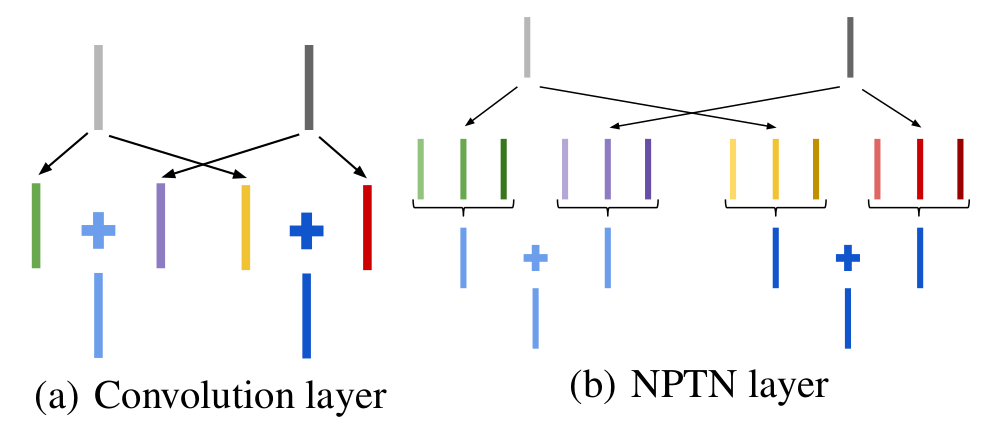
\includegraphics[scale=0.15]{result_images/nptn_paper.png}
	\caption{Illustration of CNNs vs. NPTNs. The structure of the NPTNs is the same as for PTNs. (Figure taken from \cite{NPTN18})}
	\label{pic:nptn}
	\end{center}
\end{figure}

\subsection{RotNets}
Rotation Networks (RotNets) were our idea for the additional task of designing a network that due to its structure is invariant to rotations. 
The idea is based on the same structure as PTNs (and NPTNs), just that the group of transformations is fixed to be rotations. Therefore there exists one set of weights $w$, which is learned for each $|G|$ transformations and this weights are rotated into the new kernels. 
\newcommand{\pytorch}{PyTorch }
\section{Implementation in \pytorch}
\newcommand{\nnaffinegrid}{\nolinkurl{nn.functional.affine\textunderscore grid} }
\newcommand{\nngridsample}{\nolinkurl{nn.functional.grid\textunderscore sample} }
\newcommand{\nnConvFunction}{\nolinkurl{nn.functional.conv2d} }
\newcommand{\nnConvLayer}{\nolinkurl{nn.Conv2d} }
\newcommand{\nnMaxPool}{\nolinkurl{nn.MaxPool3d} }
\newcommand{\nnAvgPool}{\nolinkurl{nn.AvgPool3d} }
\newcommand{\nnTensor}{\nolinkurl{nn.Tensor} }
\newcommand{\nnParameter}{\nolinkurl{torch.nn.Parameter} }

As the authors of the paper on NPTNs \cite{NPTN18} we used \pytorch for the implementation of the experiments.
To be able to reproduce the experiments performed in the paper and conduct experiments on RotNet we had to implement the NPTN layer as well as the RotNet layer.

When implementing new network architectures in \pytorch it's crucial to specify which values AutoGrad should view as parameters of the network in order for it to be able to apply backpropagation algorithm to the network. Furthermore you need to take care, that all calculations and operations performed in the forward path are differentiable by AutoGrad.
\subsection{The NPTN Layer}
%TODO Add NPTN graphics!
Our implementation follows the description given in the NPTN paper. A sketch of our implementation is given in Figure \ref{fig:NptnImplementation}.
Lets say we have $M$ inputs and want $N$ outputs while using a set of $|G|$ different filters for each path from input to output.
Just as for CNNs, all filters we use during convolution are also parameters that are expected to be learned by the network.
For this reason we can perform the convolutions by using an instance of the \nnConvLayer layer which will automatically initialize the filters and also register them as learn able parameters. This way, by using \nnConvLayer we don't need to worry about AutoGrad and differentiability of parameters ourself.

In it's constructor we specify it to have $M$ inputs and $M \cdot N \cdot |G|$ outputs. The important implementation detail here is, that we need to set the groups option to $M$, which causes \nnConvLayer to use a filter bank of $N\cdot|G|$ filters per input.

%TODO DEL USE SPACE NEEDED__ 
As stated in the \pytorch documentation \cite{PyTorchDocumentation} the output value of the \nnConvLayer layer with input size $(N, C_{in}, H, W)$ and output $(N, C_{out}, H_{out}, W_{out})$ can be precisely described as:
\begin{equation*}
\text{out}(N_i, C_{out_j}) = \text{bias}(C_{out_j}) +
\sum_{k = 0}^{C_{in} - 1} \text{weight}(C_{out_j}, k) \star \text{input}(N_i, k)
\end{equation*}
but since setting groups to $M$ causes \nnConvLayer to operate as if there are $M$ convolution layers side by side, each seeing one input channel and producing $N\cdot|G|$ output channels, $C_{in} = 1$, which means, that there will be no weighted sum since only one convolution will be calculated per output.
%TODO __DEL USE SPACE NEEDED

After calling the convolution, we have a tensor with $N$ consecutive packs of $|G|$ layers produced by the same input. But we need $|G|$ layers of input 1 to be followed by $|G|$ layers of input 2 and so on. This can be achieved by a simple permutation, which we decided to defer until after the max pooling across channels. We will come back to this permutation later.

Next we use \nnMaxPool with stride 1 and kernel size $(|G|,1,1)$. Note, that this does not resemble spatial max pooling as is commonly used in CNNs, but rather the pixel wise maximum of $|G|$ consecutive layers.

Following this, to perform the aforementioned permutation, we defined a matrix of numbers from zero to the number of layers left in the tensor, permuted it, and then indexed the tensor with it. Note, that this is valid, because indexing tensors is tracked by AutoGrad.
%TODO Maybe add: Permutation with matrix as formula.

This is followed by the average pooling across layers, which is common to CNNs and actually replaces the weighted sum operation in the formula of $\text{out}(N_i, C_{out_j})$ above. This can be archived by using \nnAvgPool.

\begin{figure}
	\begin{center}
		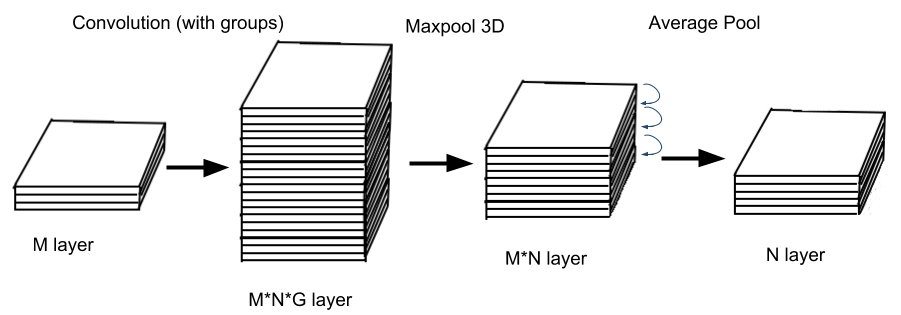
\includegraphics[width=0.75\textwidth]{result_images/NptnImplementation.png}
		\caption{A pass through the NPTN layer}
		\label{fig:NptnImplementation}
	\end{center}
\end{figure}

\subsection{The RotNet Layer}
Within the implementation of the NPTN layer we were able to use an instance of \nnConvLayer, because every kernel used for convolution was also a learnable parameter of the network.
For the RotNet layer on the other hand, where we only want to learn the unrotated kernels while performing convolution with a few rotated versions of them, we can't use \nnConvLayer class but need to use the \nnConvFunction  function instead.
This requires us to define and initialize a \nnTensor representing the unrotated kernels ourself. We also need to mark them as trainable parameters which is done by wrapping the \nnTensor into an \nnParameter object.\\
To compute the rotated versions of the kernels, we used the functions \nnaffinegrid and \nngridsample, because they are differentiable by AutoGrad while performing interpolation which allows for arbitrary rotation angles to be applied. We had to specify the rotation matrices we want to use, convert them to flow fields using \nnaffinegrid and then perform the rotations using \nngridsample. The constructor of our RotNet layer expects a parameter \nolinkurl{alpha} which tells the layer to create rotated versions of the kernel with rotation angles between \nolinkurl{-alpha} and \nolinkurl{alpha}.\\
The rest of the layer implementation, namely the \nnMaxPool, permutation of layers and the final \nnAvgPool are the same as in our NPTN implementation.

\subsection{Multi Layer Networks}


\subsubsection{Input size to fully connected layer}
The last layer of a network hierarchy usually is a fully connected layer, and \pytorch requires us to specify the dimensions of this layer on instantiation. We decided to expect the input size of the network as an argument to the networks constructor, initialize a random tensor with this specified input size, and then pass it through the network excluding the fully connected layer, in order to use the size of the result to initialize the fully connected layer. This makes it easier to change the network (e.g. kernel size, input image size, number of layers) without having to calculate and adapt the size of the fully connected layer manually. 

\subsubsection{YAML files for Experiment setup}
We had to run a lot of experiments. In order to avoid code duplication and promote code readability we parsed YAML files containing the parameters.

\section{Experiments and Results}	
In the following we will present three experiments from the paper that we tried to reproduce. 
All the experiments used a two-layered or three-layered structure. From now on (as in the paper) when we use the term layer, we refer to a structure that contains either the convolution layer, the NPTN layer or the RotNet layer, followed by other operations. The concrete design of the two-layered network is shown in Figure \ref{pic:network_structure}. The last log-softmax layer is not described in the paper, but was added by us. 
For the experiments we noticed in general that the runtime of NPTNs of RotNets was alike and slightly longer than for the CNNs. This is not surprising as the NPTNs contain the convolution operation as well as additional operations at the same place that the CNNs only perform the convolution. 
\begin{figure}
	\begin{center}
	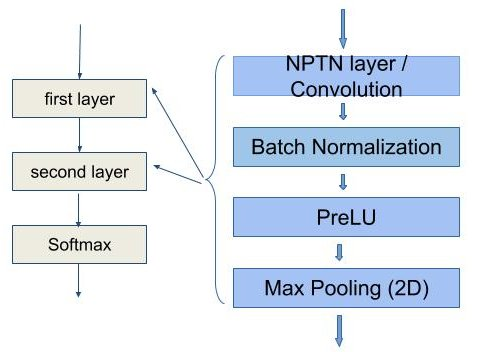
\includegraphics[scale=0.35]{result_images/network_structure.jpg}
	\caption{Structure of a two layered network.}
	\label{pic:network_structure}
	\end{center}
\end{figure}


\subsection{Experiments on CIFAR-10}
The first experiment used the CIFAR-10 dataset [CITE]. A CNN and several NPTNs with different values for $|G|$ are tested. The dimension of the NPTNs is changed for the different values of G such that all networks have the same amount of filters.
The paper describes in detail the setup of the experiments regarding learning rate, data preprocessing and network dimensions. However other important information as filter size and loss function is missing. 
For the filter size we used 5, since for the other experiments, the paper mentions  filter sizes of 3, 5 or 7 where 5 often shows the best performance for the NPTNs. 
In Figure \ref{pic:first_experiment} we show the results from the paper next to our experimental results. For the loss function we chose Negative Log Likelihood Loss (NLLL). 
Comparing the loss values of the networks to each other, in the paper, all NPTNs perform better than the CNN. In our results, only one of the NPTNs performs better.
However the loss values we obtained were to different to the ones from the paper to perform a direct comparison. 
Also we are not sure if we used the same loss as in the paper.  Therefore we also calculated the accuracy of the networks. The values are consistent with the loss for this experiment, so for each network if the loss is lower, then the accuracy is higher compared to the other networks.

One thing we noticed during this and also the following experiment, is that the test loss was consistently lower than the training loss and also the test accuracy was higher than the training accuracy, even though we used different datasets and used the same function to calculate training and test measures.

\begin{figure}
	\begin{center}
	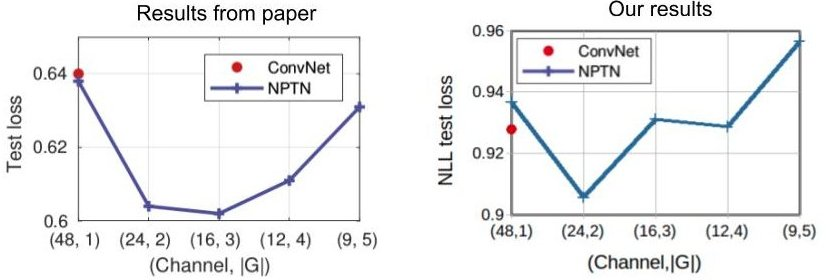
\includegraphics[scale=0.35]{result_images/experiment1.jpg}
	\caption{The first experiment}
	\label{pic:first_experiment}
	\end{center}
\end{figure}


\section{Rotation Experiments on MNIST}
The second experiment from the paper compares a CNN and several NPTNs. Again the dimensions are chosen in a way that matches the values in the paper and leads to the same amount of filters for all networks. 
This experiment uses the MNIST dataset [CITE] where data augmentation was applied to all images from training and test set by randomly rotating the images up to a certain angle $\rho$. 
The paper shows the results for different values of $\rho$. We chose to run the experiments which used the highest values for $\rho$, since the performance difference between NPTNs and CNNs was the biggest for those. Also we added RotNets for comparison.
The Paper did specify the data preprocessing in detail, but didn't give new instructions for the learning rate, so we kept the same experiment setup as in the first experiment.
The results from our experiments are shown in Figure \ref{pic:second_experiment}. 
[TODO: GRAPHIC OR TABLE WILL BE INSERTED HERE]


\begin{center}
\begin{tabular}{ |c|c|c| } 
 \hline \hline
 cell1 & cell2 & cell3 \\ 
 cell4 & cell5 & cell6 \\ 
 cell7 & cell8 & cell9 \\ 
 \hline
\end{tabular}
\end{center}



The experiments in the paper show the best results for the NPTNs with parameters $|G|=2$ or $|G|=3$. Our results show the that these values are also better than the CNN. The difference in loss is also quite similar to the one in the paper. RotNet performs worse than CNN and NPTNs. Accuracy and loss again were consistent. 

\section{Three-layered networks}
This experiment from the paper compares three-layered NPTNs and CNNs on the CIFAR-10 [CITE] dataset. 
The network dimensions are not described well and the paper states that the amount of parameters for those networks is similar, but not exactly the same as in the previous experiments. 
Therefore we determined possible dimensions for the amount of channels in the NPTNs and CNNs. 
Again no new learning rate was given for this experiment, so we initially tried with the same experimental setup as in the first two experiments, but using this the networks overfit greatly and the loss values did not improve. 
Therefore we reduced the learning rate and achieved a result, which had less generalization error. 
Different than in the first two experiments accuracy and loss are not consistent anymore. While the loss starts getting worse after some iteration, the accuracy stays approximately stable and we therefore used the accuracy to compare the networks.
[GRAPHIC will be inserted HERE]
The paper achieves a lower test loss compared to the experiment with the two-layered network. Also the NPTNs with a higher value of $|G|$ have a bigger improvement compared to their baseline CNN. Our results show the opposite: All NPTNs perform worse than the CNN and they perform worse, the bigger $|G|$ is.
So many parameters on how to perform this experiment needed to be set by us, since they were not mentioned in the paper, that it is not comparable to the paper anymore.

\begin{figure}
	\begin{center}
	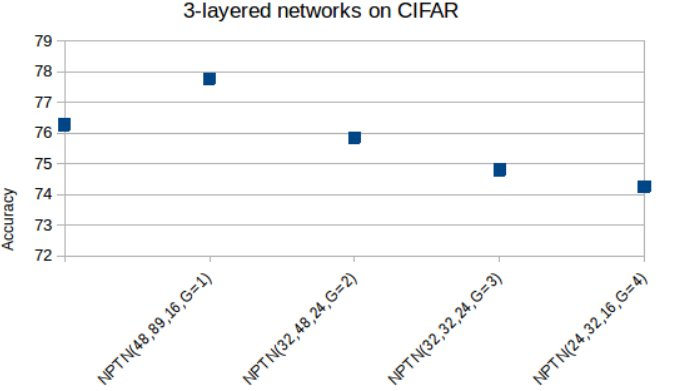
\includegraphics[scale=0.35]{result_images/experiment3.jpg}
	\caption{Accuracy of the three-layered networks on  the CIFAR-10 dataset.}
	\label{pic:experiment3}
	\end{center}
\end{figure}

\section{Experiments for RotNet}
The final experiment was designed by us to see if RotNet was able to perform one of the ideas behind its design: the ability to be invariant to rotations without learning them. [Maybe already say this in theory part] For this we copied the setup of the MNIST rotation experiment with the difference, that this time we only rotated the test set. The results are shown in Figure \ref{pic:experiment4}. 


\begin{figure}
	\begin{center}
	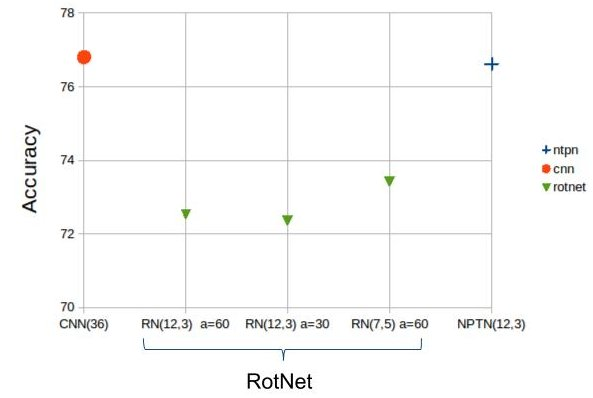
\includegraphics[scale=0.35]{result_images/experiment4.jpg}
	\caption{Results of the experiment designed for testing the ability of the networks to handle rotations that only appear in the test set.}
	\label{pic:experiment4}
	\end{center}
\end{figure}



\section{Discussion and further work}
Some of the NPTNs perform better than the CNN. However the difference is not as prominent as in the paper. Since the runtime of the NPTNs is slightly higher than that of the CNNs, CNNs might be able to achieve better results in the same runtime.

Overall it was difficult to compare our results to the paper, because important information is missing. 
RotNet performed worse than the NPTNs and the CNNs in all experiments.
It also did not show the expected advantages for handling rotated data, without learning these rotations first. 

WHY WE THINK NPTNS ARE LESS POWERFULL WHY ROTNETS ARE
WORSE THAN NPTNs WHY IT IS MAYBE NOT A GOOD IDEA TO RO-
TATE EARLY FILTERs

\section{What we learned}
In this lab we learned much about the theory of CNNs 
Dealing with tensor dimensions.
Implement networks architectures using \pytorch.

% ---- Bibliography ----
%TODO References to add:
% Figures
%   Convolution: https://arxiv.org/abs/1603.07285v2

\printbibliography
\end{document}
